\documentclass[10pt]{article}

\usepackage{geometry}
\geometry{margin = 3em,top =6em, headheight=\paperheight}
\usepackage[export]{adjustbox}
\usepackage{array}
\usepackage{amsmath}
\usepackage{amsfonts}
\usepackage{fancyhdr}
\pagestyle{fancy}
\fancyhf{}
\lhead{Algebra II}
\chead{Function Vocabulary}
\rhead{In-class Practices, Page \thepage}
\usepackage{lastpage}
\usepackage{xcolor}
\usepackage{enumitem}
\usepackage{pifont}
\usepackage{graphicx}
\graphicspath{{../img}}
\usepackage{pgfplots}
\pgfplotsset{compat=1.18}

\newcommand{\R}{\mathbb R}
\newcommand{\e}{{\rm e}}
\newcommand{\pobr}[1]{\left\langle#1\right\rangle}
\newcommand{\norm}[1]{\lVert #1 \rVert}
\newcommand{\abs}[1]{\lvert #1 \rvert}

\DeclareMathOperator{\xd}{d\!}
\DeclareMathOperator{\proj}{proj}

\title{}
\date{}

\begin{document}
{\noindent\bf Do Now.}

{\it
Terminology Review:
\begin{itemize}[leftmargin=4em]
\item
Zeros/X-Intercepts: Where the graph crosses the x-axis. 
\item
Y-Intercepts: Where the graph crosses the y-intercepts.
\end{itemize}
}
Let \(f(x) = 2x -3\). Find the zeros and the $y$-intercept of the graph of $f(x)$, then plot the graph.
\vspace{\stretch{1}}

{\noindent\bf Discussion.}

Let \(f(x) = x^2 - 6x +8\).  Find the zeros, the $y$-intercept and the vertex of the graph of $f(x)$, then plot the graph.
\vspace{\stretch{1}}

{\noindent\bf Exit Tickets.}

Describe the following graph.
\vspace{1em}

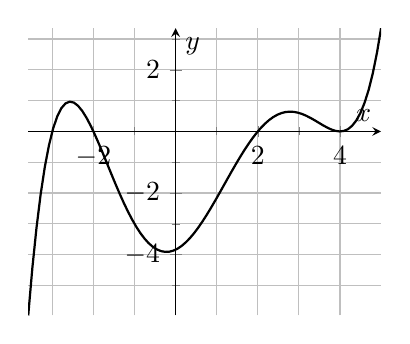
\begin{tikzpicture}
\begin{axis}[
    xlabel={$x$},
    ylabel={$y$},
    grid=both,
    minor tick num=1,
    axis lines=middle,
    domain=-5:5,
    restrict y to domain=-6:6,
    samples=100,
    width=.5\textwidth,
]
\addplot[thick] {(x+3)*(x+2)*(x-2)*(x-4)^2/50};
\end{axis}
\end{tikzpicture}

\end{document}